%===========================
% Chapitre 1 : Introduction to Supervised Learning
%===========================
\chapter{Introduction à l'Apprentissage Supervisé}

\section{Introduction}

\subsection{Objectif}

L'objectif est de construire une fonction de décision automatique basée sur des données étiquetées $D_n$, telle que $f(X)$ soit une prédiction précise de la sortie associée $Y$. Nous voulons que la prédiction $\hat{f}(X)$ soit la plus proche possible de $Y$.

\subsection{Données Étiquetées (Labeled Data)}

\begin{definition}[Échantillon d'apprentissage]
L'échantillon d'apprentissage (learning sample), noté $D_{n}$, est défini par :
\begin{equation}
D_{n}:=\{(X_{i},Y_{i})\}_{i=1}^{n}
\end{equation}
Il est composé de copies i.i.d. de la paire aléatoire $(X, Y)$. Lorsque la fonction de prédiction dépend de l'échantillon d'apprentissage, on utilise la notation $\hat{f}$ ou $\hat{f}_n$.
\end{definition}

\begin{remarque}[Notations]
Dans tout ce cours, $n$ désignera la taille de l'échantillon d'apprentissage, $d$ la dimension de l'espace d'entrée (features), $\mathcal{X} = \R^d$ l'espace des entrées et $\mathcal{Y}$ l'espace des sorties (labels).
\end{remarque}

\subsection{Pourquoi l'Apprentissage Supervisé ?}

La motivation réside dans le fait que, dans de nombreuses applications, la sortie réelle associée à une entrée $X$ n'est pas disponible, et son acquisition peut être coûteuse ou chronophage.

\subsection{Fonctions de Prédiction}

\begin{definition}[Fonction de prédiction]
Une fonction de prédiction $f$ est une fonction mesurable qui fait correspondre l'espace des caractéristiques (feature space) à l'espace de sortie :
\begin{equation}
f:\R^d\longrightarrow\mathcal{Y}, \quad x\mapsto f(x)
\end{equation}
L'ensemble de toutes les fonctions de prédiction est noté $\mathcal{F}(\R^d,\mathcal{Y})$.
\end{definition}

\begin{itemize}
    \item \textbf{Régression :} L'espace de sortie est $\mathcal{Y}=\R$.
    \item \textbf{Classification :} L'espace de sortie est fini, typiquement $\mathcal{Y}=\{1,...,K\}$. En classification binaire, $\mathcal{Y}=\{0,1\}$ ou $\mathcal{Y}=\{-1,+1\}$.
\end{itemize}

\subsection{Perte et Risque (Loss and Risk)}

\begin{definition}[Fonction de perte et risque]
Une fonction de perte (loss function) est une application :
\begin{equation}
L:\mathcal{Y}\times\mathcal{Y}\longrightarrow\R_{+}, \quad (y,y^{\prime})\mapsto L(y,y^{\prime})
\end{equation}
Étant donné une fonction de perte $L$, le risque d'une fonction de prédiction $f$ est défini comme :
\begin{equation}
R(f) = \E[L(f(X),Y)]
\end{equation}
\end{definition}

\subsection{Exemples de Fonctions de Perte}

\begin{exemple}[Fonctions de perte courantes]
\begin{itemize}
    \item \textbf{Régression :} La perte quadratique $L(y,y^{\prime})=(y-y^{\prime})^{2}$. Elle pénalise fortement les grandes erreurs, ce qui est adapté aux problèmes d'estimation continue.
    \item \textbf{Classification :} La perte 0-1 définie par $L(y,y^{\prime})=\indic_{\{y\ne y^{\prime}\}}$. Elle compte simplement le nombre d'erreurs de classification, sans distinction de magnitude.
\end{itemize}
\end{exemple}

\subsection{Prédicteur de Bayes}

\begin{definition}[Prédicteur de Bayes]
Le prédicteur de Bayes (prédicteur optimal) est défini par :
\begin{equation}
f^{*}\in \argmin_{f\in\mathcal{F}}R(f)
\end{equation}
Il satisfait $\forall f\in\mathcal{F}, R(f^{*})\le R(f)$.
\end{definition}

\subsection{Risque en Excès (Excess Risk)}

\begin{definition}[Risque en excès]
Le risque en excès d'un prédicteur $f$ est défini par :
\begin{equation}
\mathcal{E}(f)=R(f)-R(f^{*})
\end{equation}
La consistance d'un prédicteur dépendant des données $\hat{f}$ signifie que $\E[\mathcal{E}(\hat{f})]\xrightarrow[n\rightarrow\infty]{} 0$.
\end{definition}

\begin{remarque}
Le risque en excès est toujours non-négatif : $\mathcal{E}(f) \ge 0$ pour tout $f$, car $f^*$ minimise $R$ par définition.
\end{remarque}

\subsection{Caractère Aléatoire du Risque}

Le risque d'un prédicteur dépendant des données $\hat{f}$ est une variable aléatoire car il dépend de $D_n$ :
\begin{equation}
R(\hat{f})=\E[L(\hat{f}(X),Y)|D_{n}]
\end{equation}


%---------------------------
\section{Régression}
%---------------------------

En régression, $Y \in \R$ et $Y \in L^2$ ($\E[Y^2] < +\infty$). On utilise généralement la perte carrée.

\subsection{Prédicteur de Bayes et risque en excès}

\begin{proposition}[Prédicteur de Bayes en régression]
Le risque est $R(f)=\E[(Y-f(X))^{2}]$. Le prédicteur de Bayes est :
\begin{equation}
f^{*}(X)=\E[Y|X]
\end{equation}
Pour tout $f$, le risque en excès est $\mathcal{E}(f) = \E[(f(X)-f^{*}(X))^{2}]$.
\end{proposition}

\begin{proof}
Montrons que $\mathcal{E}(f) = \E[(f(X)-f^{*}(X))^{2}]$. On a :
\begin{align*}
R(f) - R(f^*) &= \E[(Y-f(X))^2] - \E[(Y-f^*(X))^2] \\
&= \E[(Y-f(X))^2 - (Y-f^*(X))^2]
\end{align*}
En utilisant l'identité $a^2 - b^2 = (a-b)(a+b)$ avec $a = Y - f(X)$ et $b = Y - f^*(X)$ :
\begin{align*}
&= \E[(f^*(X) - f(X))(2Y - f^*(X) - f(X))]
\end{align*}
Par la loi des espérances itérées, conditionnons par rapport à $X$ :
\begin{align*}
&= \E\big[\E[(f^*(X) - f(X))(2Y - f^*(X) - f(X)) \mid X]\big]
\end{align*}
Puisque $f(X)$ et $f^*(X)$ sont mesurables par rapport à $X$ :
\begin{align*}
&= \E\big[(f^*(X) - f(X)) \cdot \E[2Y - f^*(X) - f(X) \mid X]\big] \\
&= \E\big[(f^*(X) - f(X)) \cdot (2\E[Y|X] - f^*(X) - f(X))\big]
\end{align*}
Or $f^*(X) = \E[Y|X]$, donc :
\begin{align*}
&= \E\big[(f^*(X) - f(X)) \cdot (2f^*(X) - f^*(X) - f(X))\big] \\
&= \E\big[(f^*(X) - f(X))^2\big]
\end{align*}
\end{proof}

\subsection{Modèle de régression avec bruit}

\begin{proposition}[Décomposition avec bruit]
On peut écrire $Y = f^{*}(X) + \epsilon$, où $\epsilon = Y - f^*(X)$ satisfait $\E[\epsilon|X]=0$.
\end{proposition}

\begin{proof}
Posons $\epsilon = Y - f^*(X) = Y - \E[Y|X]$. Alors :
\[
\E[\epsilon | X] = \E[Y - \E[Y|X] | X] = \E[Y|X] - \E[Y|X] = 0
\]
\end{proof}

\begin{exemple}[Modèle de bruit gaussien]
On suppose que 
\[
Y = f^*(X) + \epsilon
\]
avec $\epsilon \perp X$, satisfaisant
\[
\E[\epsilon | X] = \E[\epsilon]
\]
et
\[
\epsilon \sim \mathcal{N}(0, \sigma^2).
\]
Ce modèle est appelé \textbf{modèle de bruit gaussien homoscédastique}.
\end{exemple}

\subsection{Régression Linéaire Gaussienne}

Si l'on suppose $f^{*}(X) = \langle X, \theta^* \rangle$, on obtient le modèle de régression linéaire gaussienne :
\[
Y = \langle X, \theta^* \rangle + \epsilon, \quad \epsilon \sim \mathcal{N}(0, \sigma^2)
\]

\subsection{Minimisation du Risque Empirique (ERM)}

\begin{definition}[Minimisation du risque empirique]
Le principe de l'ERM consiste à minimiser le risque empirique défini sur un échantillon $D_n$:
\begin{equation}
\hat{R}(f)=\frac{1}{n}\sum_{i=1}^{n}(Y_{i}-f(X_{i}))^{2}
\end{equation}
Le minimiseur du risque empirique sur une classe de modèles $\mathcal{F}$ est :
\begin{equation}
\hat{f} \in \argmin_{f\in\mathcal{F}}\hat{R}(f)
\end{equation}
\end{definition}

\subsection{Surapprentissage (Overfitting) et Choix de Modèle}

Restreindre la classe d'hypothèses permet d'éviter le surapprentissage (overfitting). Un modèle trop complexe peut interpoler parfaitement les données ($\hat{R}(\hat{f})=0$) mais avoir de mauvaises performances de généralisation.

\begin{exemple}[Interpolateur parfait]
Considérons la fonction $\hat{f}$ définie par :
\[
\hat{f}(x) = \begin{cases} Y_i & \text{si } x = X_i \text{ pour un } i \in \{1,\ldots,n\} \\ 0 & \text{sinon} \end{cases}
\]
Cette fonction satisfait $\hat{R}(\hat{f}) = 0$ (risque empirique nul), mais n'a aucun pouvoir de généralisation : elle prédit 0 pour toute nouvelle observation.
\end{exemple}


\begin{figure}[H]
    \centering
    \begin{tikzpicture}[scale=1.2]
        % Axes
        \draw[->, thick] (-0.5,0) -- (8,0) node[right] {$x$};
        \draw[->, thick] (0,-0.5) -- (0,5) node[above] {$y$};
        
        % True function f* (dashed line)
        \draw[gray, dashed, thick] (0.5,0.8) -- (7.5,4.2);
        \node[gray] at (7.8,4.5) {$f^*(x) = \E[Y|X]$};
        
        % Data points
        \filldraw[black] (1,1.2) circle (2pt);
        \filldraw[black] (2.5,2.3) circle (2pt);
        \filldraw[black] (3.5,2.1) circle (2pt);
        \filldraw[black] (5,3.5) circle (2pt);
        \filldraw[black] (6,3.2) circle (2pt);
        \filldraw[black] (7,4.5) circle (2pt);
        
        % Overfitting function (connects all points with zigzag)
        \draw[thick, black] (1,1.2) -- (2.5,2.3) -- (3.5,2.1) -- (5,3.5) -- (6,3.2) -- (7,4.5);
        
        % Label for overfitting function
        \node[right] at (6.5,3.8) {$\hat{f}$ that overfits};
        
        % Example point with vertical dashed line
        \draw[dashed, gray] (2.5,0) -- (2.5,2.3);
        \node[below] at (2.5,0) {$(x_i, y_i)$};
    \end{tikzpicture}
    \caption{Illustration du surapprentissage : $\hat{f}$ interpole parfaitement les données mais s'éloigne de $f^* = \E[Y|X]$.}
    \label{fig:overfitting}
\end{figure}

\begin{remarque}[Prédicteur Oracle et prédicteur ERM]
Introduisons :
\begin{equation}
\tilde{f} \in \argmin_{f \in \mathcal{F}} R(f), \qquad \hat{f} \in \argmin_{f \in \mathcal{F}} \hat{R}(f).
\end{equation}
L'oracle $\tilde{f}$ est le meilleur prédicteur \emph{possible} dans la classe $\mathcal{F}$ (mais inaccessible car $R$ est inconnu), tandis que $\hat{f}$ est le meilleur prédicteur \emph{observable} basé sur les données.
\end{remarque}

On a alors la décomposition :
\begin{equation}
\mathcal{E}(\hat{f}) = R(\hat{f}) - R(f^{*}) = \big(R(\hat{f}) - R(\tilde{f})\big) + \big(R(\tilde{f}) - R(f^{*})\big)
\end{equation}

\subsection{Décomposition Biais-Variance (Bias-Variance decomposition)}

\begin{theoreme}[Décomposition biais-variance]
Le risque en excès peut être décomposé en :
\begin{equation}
\mathcal{E}(\hat{f}) = \underbrace{(R(\hat{f})-R(\tilde{f}))}_{\text{Estimation (variance)}} + \underbrace{(R(\tilde{f})-R(f^{*}))}_{\text{Approximation (biais)}}
\end{equation}
où $\tilde{f}$ est l'oracle de la classe de modèles.
\end{theoreme}

\begin{remarque}
\begin{itemize}
    \item Le terme de \textbf{variance} (estimation) dépend de $n$ et tend vers 0 quand $n \to \infty$.
    \item Le terme de \textbf{biais} (approximation) est déterministe et dépend uniquement du choix de la classe $\mathcal{F}$.
    \item Un bon compromis biais-variance est essentiel pour une bonne généralisation.
\end{itemize}
\end{remarque}

\subsection{Estimateur des k-Plus Proches Voisins (k-NN)}

\begin{definition}[Estimateur k-NN]
Le prédicteur k-NN à un point $x$ est la moyenne des sorties des $k$ voisins les plus proches:
\begin{equation}
\hat{f}(x)=\frac{1}{k}\sum_{j=1}^{k}Y_{(j)}(x)
\end{equation}
où $Y_{(1)}(x), \ldots, Y_{(k)}(x)$ sont les sorties correspondant aux $k$ plus proches voisins de $x$ dans $D_n$.
\end{definition}


\begin{exemple}[Illustration : Points de données dans $\R^2$]
Considérons un ensemble de points dans $\R^2$. Soit $X_i = (x_i^1, x_i^2)$ des vecteurs pour $i = 1, \ldots, n$ avec $n = 5$. L'échantillon d'apprentissage est noté :
\[
\mathcal{D}_5 = \{(X_1, Y_1), \ldots, (X_5, Y_5)\}
\]
Fixons le paramètre $k = 3$.

\begin{figure}[H]
    \centering
    \begin{tikzpicture}[scale=1.0]
        % Axes
        \draw[->, thick] (-0.5,0) -- (7,0) node[right] {$x^1$};
        \draw[->, thick] (0,-0.5) -- (0,5.5) node[above] {$x^2$};
        
        % Data points (blue filled circles)
        \filldraw[blue!70!black] (2,3.8) circle (3pt) node[above right] {$x_1$};
        \filldraw[blue!70!black] (4,4.5) circle (3pt) node[above right] {$x_2$};
        \filldraw[blue!70!black] (1,1.5) circle (3pt) node[below left] {$x_3$};
        \filldraw[blue!70!black] (4,1.8) circle (3pt) node[below right] {$x_4$};
        \filldraw[blue!70!black] (3,2.8) circle (3pt) node[above right] {$x_5$};
        
        % Query point x (red cross)
        \draw[red!70!black, thick] (2.5,2) -- ++(0.2,0.2);
        \draw[red!70!black, thick] (2.5,2) -- ++(-0.2,-0.2);
        \draw[red!70!black, thick] (2.5,2) -- ++(0.2,-0.2);
        \draw[red!70!black, thick] (2.5,2) -- ++(-0.2,0.2);
        \node[red!70!black, below] at (2.5,1.8) {$x$};
        
        % Query point x' (red cross)
        \draw[red!70!black, thick] (3.2,3.5) -- ++(0.2,0.2);
        \draw[red!70!black, thick] (3.2,3.5) -- ++(-0.2,-0.2);
        \draw[red!70!black, thick] (3.2,3.5) -- ++(0.2,-0.2);
        \draw[red!70!black, thick] (3.2,3.5) -- ++(-0.2,0.2);
        \node[red!70!black, above] at (3.2,3.7) {$x'$};
    \end{tikzpicture}
\end{figure}

Les estimateurs $\hat{f}$ aux points $x$ et $x'$ sont calculés en moyennant les valeurs $Y$ des $k=3$ plus proches voisins :
\begin{align}
\hat{f}(x) &= \frac{1}{3}(Y_3 + Y_4 + Y_5) \\
\hat{f}(x') &= \frac{1}{3}(Y_1 + Y_2 + Y_5)
\end{align}
Le prédicteur $\hat{f}(x)$ effectue donc une moyenne locale des labels des voisins les plus proches. En classification, cela reviendrait à un vote majoritaire parmi les voisins.
\end{exemple}

\begin{proposition}[Taux de convergence k-NN]
Sous des hypothèses de régularité (Lipschitz), si $k \to \infty$ et $k/n \to 0$, le risque en excès suit le taux :
\begin{equation}
\E[\mathcal{E}(\hat{f})]\le Cn^{-\frac{2}{2+d}}
\end{equation}
\end{proposition}

\begin{remarque}
Ce taux souffre de la \textbf{malédiction de la dimensionnalité} : quand $d$ augmente, le taux de convergence se dégrade considérablement.
\end{remarque}

\subsection{Autres méthodes populaires}

Parmi les autres méthodes de régression/classification supervisée, on peut citer :
\begin{itemize}
    \item \textbf{Random Forests} : Agrégation d'arbres de décision
    \item \textbf{Boosting} (AdaBoost, Gradient Boosting) : Construction séquentielle de modèles faibles
    \item \textbf{Support Vector Machines (SVM)} : Maximisation de la marge
    \item \textbf{Réseaux de neurones} : Modèles à couches multiples
\end{itemize}

%---------------------------
\section{Classification}
%---------------------------

En classification multiclasse, $Y \in \{1,...,K\}$. Le risque de mauvaise classification est $R(f) = \PP(f(X) \ne Y)$.

\subsection{Prédicteur de Bayes}

\begin{definition}[Probabilités a posteriori]
On définit les probabilités a posteriori :
\begin{equation}
P_{k}(x) := \PP(Y=k|X=x)
\end{equation}
\end{definition}

\begin{proposition}[Prédicteur de Bayes en classification]
Le prédicteur de Bayes est :
\begin{equation}
f^{*}(x)\in \argmax_{k\in\{1,...,K\}}P_{k}(x)
\end{equation}
\end{proposition}

\begin{proof}
Pour tout classifieur $f$, on a :
\begin{align*}
\PP(f(X) = Y) &= \E[\indic_{\{f(X)=Y\}}] = \E\big[\E[\indic_{\{f(X)=Y\}} | X]\big] \\
&= \E\left[\sum_{k=1}^K \indic_{\{f(X)=k\}} \PP(Y=k|X)\right] \\
&= \E\left[\sum_{k=1}^K \indic_{\{f(X)=k\}} P_k(X)\right]
\end{align*}
Pour $X$ fixé, $f(X) \in \{1, \ldots, K\}$ donc un seul terme de la somme est non nul :
\[
\sum_{k=1}^K \indic_{\{f(X)=k\}} P_k(X) = P_{f(X)}(X)
\]
Cette quantité est maximisée quand $f(X)$ choisit le $k$ qui maximise $P_k(X)$, c'est-à-dire quand $f = f^*$. Donc $\PP(f^*(X) = Y) \ge \PP(f(X) = Y)$ pour tout $f$, i.e., $R(f^*) \le R(f)$.
\end{proof}

\subsection{Classification Binaire}

Si $Y \in \{0,1\}$, on définit la fonction de régression $\eta(X) := \PP(Y=1|X) = \E[Y|X]$. Le classifieur de Bayes devient :
\begin{equation}
f^{*}(x)=\indic\{\eta(x)\ge 1/2\}
\end{equation}

\begin{proposition}[Risque en excès en classification binaire]
Le risque en excès s'exprime par :
\begin{equation}
\mathcal{E}(f)=\E[|2\eta(X)-1|\indic_{\{f(X)\ne f^{*}(X)\}}]
\end{equation}
\end{proposition}

\begin{proof}
Procédons par disjonction de cas. Pour $x$ fixé, calculons $\PP(f(x) \ne Y | X=x) - \PP(f^*(x) \ne Y | X=x)$.

\textbf{Cas 1 :} $f(x) = f^*(x)$. Alors la différence est nulle.

\textbf{Cas 2 :} $f(x) \ne f^*(x)$ et $\eta(x) \ge 1/2$ (donc $f^*(x) = 1$, $f(x) = 0$).
\begin{align*}
\PP(f(x) \ne Y | X=x) - \PP(f^*(x) \ne Y | X=x) &= \PP(Y=1|X=x) - \PP(Y=0|X=x) \\
&= \eta(x) - (1-\eta(x)) = 2\eta(x) - 1
\end{align*}

\textbf{Cas 3 :} $f(x) \ne f^*(x)$ et $\eta(x) < 1/2$ (donc $f^*(x) = 0$, $f(x) = 1$).
\begin{align*}
\PP(f(x) \ne Y | X=x) - \PP(f^*(x) \ne Y | X=x) &= \PP(Y=0|X=x) - \PP(Y=1|X=x) \\
&= (1-\eta(x)) - \eta(x) = 1 - 2\eta(x)
\end{align*}

Dans les deux cas où $f(x) \ne f^*(x)$, la différence vaut $|2\eta(x) - 1|$. D'où :
\[
\mathcal{E}(f) = \E[|2\eta(X)-1|\indic_{\{f(X)\ne f^{*}(X)\}}]
\]
\end{proof}

\subsection{Régression Logistique}

\begin{definition}[Régression logistique]
En régression logistique, on paramètre la fonction de régression $\eta(X)$ via une fonction sigmoïde :
\begin{equation}
\eta(X) = \sigma(h^*(X)) = \frac{1}{1 + \exp(-h^*(X))}
\end{equation}
où typiquement $h^*(X) = \langle X, \theta^* \rangle$ pour un certain vecteur de paramètres $\theta^* \in \R^d$.
\end{definition}

\begin{remarque}
La régression logistique est un modèle \textbf{discriminatif} : on modélise directement $\PP(Y|X)$ sans passer par la distribution jointe.
\end{remarque}

\subsection{Modèle de Mélange Gaussien (GMM)}

\begin{definition}[Modèle de mélange gaussien]
Dans ce modèle, les classes ont des probabilités a priori $\pi_k = \PP(Y=k)$ et les caractéristiques suivent une loi normale par classe : 
\begin{equation}
X|Y=k \sim \mathcal{N}_{d}(\mu_{k},\Sigma_{k})
\end{equation}
\end{definition}

\begin{proposition}[Prédicteur de Bayes pour GMM]
Le prédicteur de Bayes est :
\begin{equation}
g^{*}(x)\in \argmax_{k\in\{1,...,K\}} \pi_{k}\varphi_{d}(x;\mu_{k},\Sigma_{k})
\end{equation}
où $\varphi_d$ désigne la densité de la loi normale multivariée.
\end{proposition}

\begin{proof}
Par la règle de Bayes :
\[
\PP(Y=k | X=x) = \frac{\PP(X=x | Y=k) \cdot \PP(Y=k)}{\PP(X=x)} = \frac{\varphi_d(x; \mu_k, \Sigma_k) \cdot \pi_k}{\varphi_X(x)}
\]
où la densité marginale de $X$ est donnée par :
\[
\varphi_X(x) = \sum_{j=1}^K \pi_j \varphi_d(x; \mu_j, \Sigma_j)
\]
Ainsi, le classifieur de Bayes $f^*(x)$ maximise le numérateur :
\[
f^*(x) \in \argmax_{k \in \{1,\ldots,K\}} \frac{\pi_k \varphi_d(x; \mu_k, \Sigma_k)}{\sum_{j=1}^K \pi_j \varphi_d(x; \mu_j, \Sigma_j)}
\]
Ce qui revient à maximiser $\pi_k \varphi_d(x; \mu_k, \Sigma_k)$.
\end{proof}

\begin{remarque}
Le GMM est un modèle \textbf{génératif} : on modélise la distribution jointe $\PP(X, Y) = \PP(X|Y)\PP(Y)$.
\end{remarque}

\subsubsection{Approche Plug-in et Analyse Discriminante de Fisher}

Dans la pratique, les paramètres $(\pi_k)_k, (\mu_k)_k, (\Sigma_k)_k$ sont inconnus. Nous ne pouvons pas calculer directement $f^*$. Nous devons estimer $f^*$ par $\hat{f}$ à partir de l'échantillon d'apprentissage $D_n$.

\begin{definition}[Plug-in approach]
L'approche "plug-in" consiste à considérer des estimateurs $\hat{\pi}_k, \hat{\mu}_k, \hat{\Sigma}_k$ des paramètres inconnus, calculés sur $D_n$, et à les substituer dans l'expression du prédicteur de Bayes.
\end{definition}

On construit ainsi le prédicteur :
\begin{equation}
\hat{f}(x) \in \argmax_{k \in \{1,\ldots,K\}} \frac{\hat{\pi}_k \hat{\varphi}_k(x)}{\sum_{j=1}^K \hat{\pi}_j \hat{\varphi}_j(x)}
\end{equation}
où $\hat{\varphi}_k$ est la densité de $\mathcal{N}_d(\hat{\mu}_k, \hat{\Sigma}_k)$.

\begin{remarque}[LDA vs QDA]
Distinguer deux cas :
\begin{itemize}
    \item \textbf{Cas 1 : } $\Sigma_k = \Sigma$ pour tout $k$.
    Dans ce cas, on parle de \textbf{Linear Discriminant Analysis (LDA)}. Les frontières de décision sont linéaires.
    \item \textbf{Cas 2 : } $\Sigma_k \ne \Sigma_{k'}$ pour $k \ne k'$.
    Dans ce cas, on parle de \textbf{Quadratic Discriminant Analysis (QDA)}. Les frontières de décision sont quadratiques.
\end{itemize}
\end{remarque}

\begin{exemple}[Modèle Bernoulli-Gaussien]
Illustrons ces concepts avec un exemple concret et calculable explicitement.
Considérons le cas binaire ($Y \in \{0, 1\}$) unidimensionnel ($d=1$).
Supposons que :
\[
Y \sim \mathcal{B}ern(1/2) \quad (\pi_0 = \pi_1 = 1/2)
\]
et que conditionnellement à $Y=y$, $X$ suit une loi normale :
\[
X | Y=y \sim \mathcal{N}(\mu_y, \sigma^2)
\]
avec $\mu_1 > \mu_0$ (et même variance $\sigma^2$).

On a par la formule de Bayes :
\[
\PP(Y=y | X=x) = \frac{\exp\left( - \frac{(x-\mu_y)^2}{2\sigma^2} \right)}{\exp\left( - \frac{(x-\mu_1)^2}{2\sigma^2} \right) + \exp\left( - \frac{(x-\mu_0)^2}{2\sigma^2} \right)}
\]
(car les termes $1/(\sigma\sqrt{2\pi})$ et les probabilités a priori $1/2$ se simplifient au numérateur et au dénominateur).

Le classifieur de Bayes est défini par :
\[
f^*(x) = \indic\left\{\PP(Y=1|X=x) \ge \PP(Y=0|X=x)\right\}
\]
Ainsi :
\begin{align*}
\PP(Y=1|X=x) \ge \PP(Y=0|X=x) &\iff \PP(Y=1|X=x) \ge 1 - \PP(Y=1|X=x) \\
&\iff \PP(Y=1|X=x) \ge \frac{1}{2} \\
&\iff \frac{1}{2}\exp\left( - \frac{(x-\mu_1)^2}{2\sigma^2} \right) \ge \frac{1}{2}\exp\left( - \frac{(x-\mu_0)^2}{2\sigma^2} \right) \\
&\iff - \frac{(x-\mu_1)^2}{2\sigma^2} \ge - \frac{(x-\mu_0)^2}{2\sigma^2} \\
&\iff (x-\mu_1)^2 \le (x-\mu_0)^2 \\
&\iff x^2 - 2x\mu_1 + \mu_1^2 \le x^2 - 2x\mu_0 + \mu_0^2 \\
&\iff - 2x\mu_1 + \mu_1^2 \le - 2x\mu_0 + \mu_0^2 \\
&\iff 2x\mu_1 - 2x\mu_0 \ge \mu_1^2 - \mu_0^2 \\
&\iff 2x(\mu_1 - \mu_0) \ge \mu_1^2 - \mu_0^2 \\
&\iff x(\mu_1 - \mu_0) \ge \frac{\mu_1^2 - \mu_0^2}{2} \\
&\iff x \ge \frac{\mu_1 + \mu_0}{2} \quad (\text{car } \mu_1 - \mu_0 > 0)
\end{align*}
Comme $\mu_1 > \mu_0$, le point milieu est $(\mu_0+\mu_1)/2$. La condition équivaut à $x \ge \frac{\mu_0+\mu_1}{2}$.

\textbf{Interprétation :} Puisque les variances sont identiques, la frontière de décision optimale se situe exactement au milieu du segment reliant les deux moyennes. Le modèle choisit la classe dont la moyenne est la plus proche de l'observation $x$.
\end{exemple}

\begin{remarque}[Généralisation à $\R^d$]
Ce résultat se généralise en dimension $d$. Si $\Sigma_0 = \Sigma_1 = \Sigma = I_d$ (identité), la frontière de décision est un hyperplan affine défini par :
\[
f^*(x) = \indic\left\{ x^\top (\mu_1 - \mu_0) \ge \frac{1}{2} (\|\mu_1\|^2 - \|\mu_0\|^2) \right\}
\]
\end{remarque}

\begin{exercice}[Calcul du Risque de Bayes]
Exprimer le risque de Bayes $R(f^*)$ pour cet exemple en fonction de la fonction de répartition $\Phi$ de la loi normale standard.

\textbf{Correction :}
Par définition du risque, on a :
\begin{align*}
R(f^*) &= \PP(f^*(X) \neq Y) \\
&= \PP(Y=1, f^*(X)=0) + \PP(Y=0, f^*(X)=1) \\
&= \PP(Y=1) \PP(f^*(X)=0 | Y=1) + \PP(Y=0) \PP(f^*(X)=1 | Y=0)
\end{align*}
Comme $\PP(Y=1) = \PP(Y=0) = 1/2$, on obtient :
\begin{align*}
\PP(f^*(X)=0 | Y=1) &= \PP\left( X < \frac{\mu_1+\mu_0}{2} \bigg| Y=1 \right) \\
&= \PP\left( \frac{X-\mu_1}{\sigma} < \frac{\frac{\mu_1+\mu_0}{2} - \mu_1}{\sigma} \bigg| Y=1 \right) \\
&= \PP\left( Z < \frac{\mu_0-\mu_1}{2\sigma} \right) \quad \text{où } Z \sim \mathcal{N}(0,1) \\
&= \Phi\left( \frac{\mu_0-\mu_1}{2\sigma} \right)
\end{align*}
où $\Phi$ est la fonction de répartition (c.d.f.) de la loi $\mathcal{N}(0,1)$.

De même, par symétrie :
\[
\PP(f^*(X)=1 | Y=0) = \PP\left( X \ge \frac{\mu_1+\mu_0}{2} \bigg| Y=0 \right) = \Phi\left( \frac{\mu_0-\mu_1}{2\sigma} \right)
\]
Ainsi, le risque de Bayes est :
\[
R(f^*) = \Phi\left( \frac{\mu_0-\mu_1}{2\sigma} \right) = \Phi\left( - \frac{\mu_1-\mu_0}{2\sigma} \right)
\]
Or, on sait que $\forall z \in \R, \Phi(z) + \Phi(-z) = 1$. D'où :
\[
R(f^*) = 1 - \Phi\left( \frac{\mu_1-\mu_0}{2\sigma} \right)
\]
\end{exercice}

\begin{exercice}[Généralisation à $\R^d$]
Généraliser l'expression du risque de Bayes obtenue ci-dessus au cas multidimensionnel où $\mu_1, \mu_0 \in \R^d$ et $\Sigma = I_d$.

\textbf{Correction :}
Dans le cas $\Sigma = I_d$, la frontière de décision est l'hyperplan médiateur du segment $[\mu_0, \mu_1]$. Le problème est invariant par rotation et dépend uniquement de la distance entre les moyennes projetée sur le vecteur discriminant $w = \mu_1 - \mu_0$.
Le problème se ramène à un cas unidimensionnel le long de l'axe défini par $\mu_1 - \mu_0$. La distance effective entre les deux centres est $\|\mu_1 - \mu_0\|$.
Par analogie avec le cas 1D où la distance était $|\mu_1 - \mu_0|$, le risque de Bayes devient :
\[
R(f^*) = 1 - \Phi\left( \frac{\|\mu_1-\mu_0\|}{2\sigma} \right)
\]
\end{exercice}

\section{Analyse Générale du Classifieur Plug-in}

Cette section formalise l'approche du "Plug-in Classifier" pour construire un classifieur à partir des données.

\subsection{Définition et Approche}

Supposons que la distribution conjointe $(X, Y)$ soit inconnue.
Le classifieur de Bayes est donné par :
\[
f^*(x) \in \argmax_{k \in \{1, \dots, K\}} P_k(x)
\]
où $P_k(x) = \mathbb{P}(Y=k | X=x)$.

Le \textbf{Classifieur Plug-in} $\hat{f}$ est défini en remplaçant les probabilités réelles $P_k$ par des estimateurs $\hat{P}_k$ construits à partir des données :
\[
\hat{f}(x) \in \argmax_{k \in \{1, \dots, K\}} \hat{P}_k(x)
\]
où $\hat{P}_k$ est un estimateur de $P_k$.

\subsection{Borne sur le Risque en Excès}

Nous avons le résultat fondamental suivant qui lie la performance du classifieur plug-in à la qualité de l'estimation des probabilités conditionnelles.

\begin{theoreme}[Borne du classifieur Plug-in]
Le risque en excès du classifieur plug-in est borné par l'erreur d'estimation $L^1$ des probabilités conditionnelles :
\[
R(\hat{f}) - R(f^*) \le \sum_{k=1}^K \mathbb{E}\left[ |\hat{P}_k(X) - P_k(X)| \right]
\]
\end{theoreme}

\begin{proof}
Considérons la différence des risques conditionnels en un point $x$. On sait que (voir section précédente) :
\[
\mathbb{P}(f^*(X) \neq Y | X=x) - \mathbb{P}(f(X) \neq Y | X=x) = P_{f(x)}(x) - P_{f^*(x)}(x)
\]
Cependant, ceci est négatif car $f^*$ est optimal. Utilisons plutôt la notation du risque en excès.
On a :
\[
R(\hat{f}) - R(f^*) = \mathbb{E}\left[ P_{f^*(X)}(X) - P_{\hat{f}(X)}(X) \right]
\]
En effet, minimiser le risque revient à maximiser la probabilité de la bonne classe.
Pour un $x$ donné, notons $k^* = f^*(x)$ et $\hat{k} = \hat{f}(x)$.
Si $k^* = \hat{k}$, la différence est nulle.
Sur l'événement $\{f^*(x) \neq \hat{f}(x)\}$, nous avons :
\begin{align*}
P_{f^*(x)}(x) - P_{\hat{f}(x)}(x) &= P_{f^*(x)}(x) - \hat{P}_{f^*(x)}(x) + \hat{P}_{f^*(x)}(x) - P_{\hat{f}(x)}(x) \\
&= \left( P_{f^*(x)}(x) - \hat{P}_{f^*(x)}(x) \right) + \left( \hat{P}_{f^*(x)}(x) - \hat{P}_{\hat{f}(x)}(x) \right) + \left( \hat{P}_{\hat{f}(x)}(x) - P_{\hat{f}(x)}(x) \right)
\end{align*}
Par définition de $\hat{f}$, $\hat{f}(x)$ maximise $\hat{P}_k(x)$, donc :
\[
\hat{P}_{\hat{f}(x)}(x) \ge \hat{P}_{f^*(x)}(x) \implies \hat{P}_{f^*(x)}(x) - \hat{P}_{\hat{f}(x)}(x) \le 0
\]
Ainsi :
\begin{align*}
P_{f^*(x)}(x) - P_{\hat{f}(x)}(x) &\le P_{f^*(x)}(x) - \hat{P}_{f^*(x)}(x) + \hat{P}_{\hat{f}(x)}(x) - P_{\hat{f}(x)}(x) \\
&\le |P_{f^*(x)}(x) - \hat{P}_{f^*(x)}(x)| + |\hat{P}_{\hat{f}(x)}(x) - P_{\hat{f}(x)}(x)| \\
&\le \sum_{k=1}^K |P_k(x) - \hat{P}_k(x)|
\end{align*}
En prenant l'espérance, on obtient le résultat :
\[
\mathbb{E}[R(\hat{f}) - R(f^*)] \le \sum_{k=1}^K \mathbb{E}[ |\hat{P}_k(X) - P_k(X)| ]
\]
\end{proof}

\subsection{Consistance}

\begin{corollaire}[Consistance]
Si les estimateurs $\hat{P}_k$ sont consistants (i.e., convergent vers $P_k$ en probabilité ou p.s.), alors le classifieur plug-in associé $\hat{f}$ est \textbf{consistant}, c'est-à-dire :
\[
R(\hat{f}) \to R(f^*) \quad \text{quand } n \to \infty
\]
\end{corollaire}

\begin{remarque}[Cas Binaire]
Dans le cas binaire où $Y \in \{0, 1\}$, on denote souvent $\eta(x) = \mathbb{P}(Y=1|X=x)$.
Le classifieur de Bayes est $f^*(x) = \indic\{\eta(x) \ge 1/2\}$.
Le classifieur plug-in est $\hat{f}(x) = \indic\{\hat{\eta}(x) \ge 1/2\}$.
\end{remarque}

\subsection{Analyse Détaillée du Cas Binaire}

Approfondissons le cas où $\mathcal{Y}=\{0,1\}$. Soit $\hat{\eta}$ un estimateur de la fonction de régression $\eta$.
Nous avons le résultat suivant pour l'excès de risque :

\begin{proposition}[Excès de risque en classification binaire]
\[
\mathbb{E}[R(\hat{f}) - R(f^*)] = \mathbb{E}\left[ |2\eta(X) - 1| \cdot \indic_{\{\hat{f}(X) \neq f^*(X)\}} \right]
\]
\end{proposition}

\begin{proof}
Sur l'événement $\{\hat{f}(X) \neq f^*(X)\}$, on commet une erreur.
Sans perte de généralité, supposons pour un $x$ donné que $f^*(x)=1$. Cela implique que $\eta(x) \ge 1/2$.
Si $\hat{f}(x) \neq f^*(x)$, alors $\hat{f}(x)=0$, ce qui implique $\hat{\eta}(x) < 1/2$.
Dans ce cas, la différence des probabilités conditionnelles est :
\[
P_{f^*(x)}(x) - P_{\hat{f}(x)}(x) = \eta(x) - (1-\eta(x)) = 2\eta(x) - 1 = |2\eta(x)-1|
\]
De même, si $f^*(x)=0$ (donc $\eta(x) < 1/2$) et $\hat{f}(x)=1$ (donc $\hat{\eta}(x) \ge 1/2$), la différence est :
\[
P_{f^*(x)}(x) - P_{\hat{f}(x)}(x) = (1-\eta(x)) - \eta(x) = 1 - 2\eta(x) = |2\eta(x)-1|
\]
D'où le résultat en prenant l'espérance.
\end{proof}

Cette situation peut être visualisée comme suit. L'erreur se produit lorsque $\eta(x)$ et $\hat{\eta}(x)$ sont de part et d'autre du seuil $1/2$.

\begin{center}
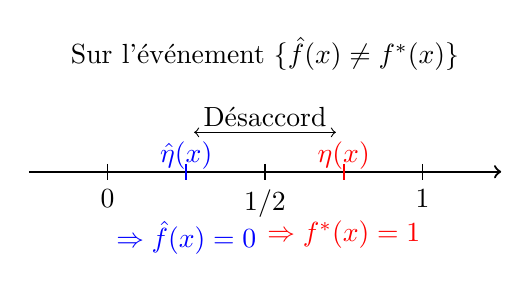
\begin{tikzpicture}
    % Droite réelle
    \draw[->, thick] (0,0) -- (6,0);
    
    % Bornes 0 et 1
    \draw (1,0.1) -- (1,-0.1) node[below] {$0$};
    \draw (5,0.1) -- (5,-0.1) node[below] {$1$};
    
    % Milieu 1/2
    \draw (3,0.1) -- (3,-0.1) node[below] {$1/2$};
    
    % Position de eta chapeau (erreur)
    \draw[blue, thick] (2,0.1) -- (2,-0.1) node[above] {$\hat{\eta}(x)$};
    \node[blue, below] at (2,-0.5) {$\Rightarrow \hat{f}(x)=0$};
    
    % Position de eta (vrai)
    \draw[red, thick] (4,0.1) -- (4,-0.1) node[above] {$\eta(x)$};
    \node[red, below] at (4,-0.5) {$\Rightarrow f^*(x)=1$};
    
    % Annotation de l'événement
    \node at (3, 1.5) {Sur l'événement $\{ \hat{f}(x) \neq f^*(x) \}$};
    \draw[<->] (2.1, 0.5) -- (3.9, 0.5);
    \node at (3, 0.7) {Désaccord};
\end{tikzpicture}
\end{center}
Sur l'événement $\{\hat{f}(x) \neq f^*(x)\}$, nous avons donc :
\[
|\hat{\eta}(x) - \eta(x)| \ge |\eta(x) - 1/2|
\]
Cela implique (en utilisant l'expression précédente de l'excès de risque) :
\[
\mathbb{E}[R(\hat{f}) - R(f^*)] = 2\mathbb{E}\left[ \left| \eta(X) - \frac{1}{2} \right| \indic_{\{\hat{f}(X) \neq f^*(X)\}} \right]
\]
En utilisant l'inégalité démontrée ci-dessus sur l'événement erreur, nous pouvons majorer ce terme :
\[
\mathbb{E}[R(\hat{f}) - R(f^*)] \le 2\mathbb{E}\left[ |\hat{\eta}(X) - \eta(X)| \indic_{\{\hat{f}(X) \neq f^*(X)\}} \right] \le 2\mathbb{E}[|\hat{\eta}(X) - \eta(X)|]
\]
Ainsi, la performance du classifieur plug-in est directement contrôlée par la qualité d'estimation $L^1$ de la fonction de régression $\eta$.

\begin{definition}[Estimateur des k-Plus Proches Voisins]
Soit $D_n = \{(X_i, Y_i)\}_{i=1}^n$ l'échantillon d'apprentissage et $k \ge 1$ un entier.
Pour tout $x \in \R^d$, considérons les données réordonnées selon la distance euclidienne $d(x,y) = \|x-y\|$, notées $X_{(1)}(x), \dots, X_{(n)}(x)$, telles que :
\[
\|X_{(1)}(x) - x\| \le \|X_{(2)}(x) - x\| \le \dots \le \|X_{(n)}(x) - x\|
\]
Soit $Y_{(i)}(x)$ l'étiquette associée à $X_{(i)}(x)$.
L'estimateur de la probabilité conditionnelle $P_j(x) = \PP(Y=j|X=x)$ est donné par la proportion de voisins de classe $j$ parmi les $k$ plus proches :
\[
\hat{P}_j(x) = \frac{1}{k} \sum_{i=1}^k \indic_{\{Y_{(i)}(x) = j\}}
\]
Le classifieur des k-NN est alors défini par le principe "Plug-in" :
\[
\hat{f}_{kNN}(x) \in \argmax_{j \in \{1,\dots,K\}} \hat{P}_j(x)
\]
\end{definition}

\begin{exemple}[Illustration k-NN ($k=3$ en $\R^2$)]
La figure suivante illustre le principe de décision pour $k=3$ dans un problème à deux classes (ronds et carrés).

\begin{center}
\begin{tikzpicture}[scale=1.5]
    % Axes
    \draw[->, thick] (-0.5,0) -- (4,0) node[below] {$x^1$};
    \draw[->, thick] (0,-0.5) -- (0,3) node[left] {$x^2$};
    
    % Données Classe 0 (Ronds)
    \foreach \point in {(0.5,2.5), (0.2,1.8), (0.8,1.2), (1.1,1.4), (2.5,2.0)} {
        \draw \point circle (2pt);
    }
    % Quelques ronds en haut à gauche
    
    % Données Classe 1 (Carrés)
    \foreach \point in {(1.5,0.8), (2.0,0.5), (2.8,0.7), (1.2,2.8), (1.8,1.1)} {
        \draw \point +(-2pt,-2pt) rectangle +(2pt,2pt);
    }
    
    % Point de test x (classifié comme Rond)
    \coordinate (X) at (0.9, 1.8);
    \node[label={above:$x$}] at (X) {$\times$};
    % Voisins de x (triche visuelle)
    \draw[dashed, red] (X) -- (0.5,2.5);
    \draw[dashed, red] (X) -- (1.1,1.4);
    \draw[dashed, red] (X) -- (0.2,1.8);
    \node[right, red] at (2.5, 2.2) {$\hat{f}_{3NN}(x) = \text{Rond}$};
    \draw[->, red, bend right] (2.5, 2.2) to (X);
    
    % Point de test x' (classifié comme Carré)
    \coordinate (Xp) at (2.2, 0.9);
    \node[label={below:$x'$}] at (Xp) {$\times$};
    % Voisins de x'
    \draw[dashed, blue] (Xp) -- (1.5,0.8);
    \draw[dashed, blue] (Xp) -- (2.0,0.5);
    \draw[dashed, blue] (Xp) -- (2.8,0.7);
    \node[right, blue] at (3, 1.2) {$\hat{f}_{3NN}(x') = \text{Carré}$};
    \draw[->, blue, bend left] (3, 1.2) to (Xp);

    % Titre
    %\node[above] at (2, 3.2) {2 classes, $k=3$, $X \in \R^2$};
\end{tikzpicture}
\end{center}
Pour le point $x$, la majorité des 3 voisins sont des ronds $\Rightarrow$ Classe "Rond".
Pour le point $x'$, la majorité des 3 voisins sont des carrés $\Rightarrow$ Classe "Carré".
\end{exemple}

\section{Minimisation du Risque Empirique (Empirical Risk Minimization)}

Le classifieur de Bayes $f^*$ est caractérisé par :
\[
f^* \in \argmin_f R(f)
\]
où $R(f) = \PP(f(X) \neq Y)$ est le risque théorique.

\subsection{Principe de l'ERM}

En pratique, le risque $R(f)$ est inconnu car la distribution $(X,Y)$ n'est pas accessible. On dispose uniquement d'un échantillon d'apprentissage $D_n = \{(X_i, Y_i)\}_{i=1}^n$.

\begin{definition}[Risque Empirique]
Soit $\mathcal{F}$ une classe de prédicteurs (modèle). Le risque empirique d'un prédicteur $f \in \mathcal{F}$ est défini par :
\[
\hat{R}(f) = \frac{1}{n} \sum_{i=1}^n \indic_{\{f(X_i) \neq Y_i\}}
\]
\end{definition}

L'estimateur par minimisation du risque empirique (ERM) est :
\[
\hat{f} \in \argmin_{f \in \mathcal{F}} \hat{R}(f) = \argmin_{f \in \mathcal{F}} \frac{1}{n} \sum_{i=1}^n \indic_{\{f(X_i) \neq Y_i\}}
\]
$\hat{f}$ est appelé \textbf{empirical risk estimator}.

\subsection{Difficultés de l'ERM}

\begin{remarque}[Deux problèmes majeurs]
L'optimisation directe de l'ERM pose deux difficultés :
\begin{enumerate}
    \item \textbf{La perte 0-1 n'est pas convexe.} La fonction indicatrice $\indic_{\{f(x) \neq y\}}$ n'est pas une fonction convexe, ce qui rend l'optimisation difficile.
    \item \textbf{L'ensemble des classifieurs n'est pas convexe.} L'espace $\mathcal{F}$ des classifieurs possibles n'a généralement pas de structure convexe.
\end{enumerate}
\end{remarque}

\subsection{Solution : Surrogate Convex}

Pour éviter ces deux problèmes, on considère une \textbf{relaxation convexe} (convex surrogate) du problème initial.

\subsubsection{Fonctions de Score}

Plutôt que de considérer directement un ensemble de classifieurs $f : \R^d \to \{1, \dots, K\}$, on considère un ensemble de \textbf{fonctions de score} :
\[
h : \R^d \to \R
\]
L'avantage est que l'ensemble des fonctions de score est un espace vectoriel : toute combinaison linéaire de fonctions de score est encore une fonction de score.

\begin{remarque}[Convexité]
Si $\lambda \in [0,1]$ et $h, h'$ sont deux fonctions de score, alors $\lambda h + (1-\lambda) h'$ est également une fonction de score. En revanche, si $f, f'$ sont deux classifieurs, $\lambda f + \mu f'$ n'est \textbf{pas} un classifieur (la somme de deux fonctions à valeurs dans $\{0,1\}$ n'est pas à valeurs dans $\{0,1\}$).
\end{remarque}

\subsubsection{Surrogate Loss Convexe}

On remplace également la perte 0-1 par une perte convexe (\textbf{surrogate loss}). Un exemple classique est la perte quadratique ($L_2$ loss) :
\[
\ell(y, y') = (y - y')^2
\]

\begin{definition}[Encodage One-Hot]
Pour la classification multiclasse avec $K$ classes, on encode les étiquettes $y \in \{1, \dots, K\}$ comme des vecteurs $Z_k \in \{-1, +1\}^K$ définis par :
\[
Z_k = 2\indic_{\{Y=k\}} - 1, \quad k \in \{1, \dots, K\}
\]
Autrement dit, $Z_k \in \{-1, +1\}$ et le vecteur complet est :
\[
Z = (Z_1, \dots, Z_K)^\top = \big(2\indic_{\{Y=1\}} - 1, \dots, 2\indic_{\{Y=K\}} - 1\big)^\top
\]
\end{definition}

\subsubsection{Vecteur de Fonctions de Score}

Considérons un vecteur de fonctions de score $\vec{h} = (h_1, \dots, h_K)$ où chaque $h_k : \R^d \to \R$ est une fonction de score.

Pour un vecteur $\vec{h}$ donné, on peut considérer son \textbf{classifieur associé} :
\[
f_{\vec{h}}(x) \in \argmax_{k \in \{1, \dots, K\}} h_k(x)
\]

\subsubsection{Risque $L_2$}

Pour un vecteur $\vec{h}$ de fonctions de score, on définit son risque $L_2$ associé :
\[
R_2(\vec{h}) = \sum_{k=1}^K \mathbb{E}\left[ (Z_k - h_k(X))^2 \right]
\]

Si on considère le risque empirique associé :
\[
\hat{R}_2(\vec{h}) = \frac{1}{n} \sum_{i=1}^n \sum_{k=1}^K (Z_k^i - h_k(X_i))^2
\]
avec $Z_k^i = 2\indic_{\{Y_i = k\}} - 1$.

On choisit un modèle $\mathcal{H}$ (un ensemble de vecteurs de fonctions de score).

\subsection{ERM avec Surrogate $L_2$}

L'estimateur par minimisation du risque empirique (ERM) est :
\[
\hat{\vec{h}} \in \argmin_{\vec{h} \in \mathcal{H}} \hat{R}_2(\vec{h})
\]
C'est la \textbf{convexification de l'ERM en classification}.

\begin{remarque}[Minimiseur du risque $L_2$]
Le minimiseur du risque $L_2$ est :
\[
\vec{h}^* \in \argmin_{\vec{h}} R_2(\vec{h})
\]
On peut calculer explicitement :
\[
h_k^*(x) = \mathbb{E}[Z_k | X=x] = 2\mathbb{E}[\indic_{\{Y=k\}} | X=x] - 1 = 2P_k(x) - 1 \quad \forall k
\]
\end{remarque}

Le classifieur associé au minimiseur est :
\begin{align*}
f_{\vec{h}^*}(x) &\in \argmax_k h_k^*(x) \\
&= \argmax_k (2P_k(x) - 1) \\
&= \argmax_k P_k(x) \\
&= f^*(x) \quad \text{p.s.}
\end{align*}

\subsection{Zhang's Lemma et Consistance}

\begin{theoreme}[Zhang's Lemma (2004) - Pour la perte $L_2$]
Pour toute fonction de score $\vec{h}$ et son classifieur associé $f_{\vec{h}}$, on a :
\[
R(f_{\vec{h}}) - R(f^*) \le \frac{1}{\sqrt{2}} \left( R_2(\vec{h}) - R_2(\vec{h}^*) \right)^{1/2}
\]
\end{theoreme}

\begin{corollaire}[Consistance via le risque surrogate]
Si $\hat{\vec{h}}$ est consistant par rapport au risque $R_2$ (i.e., $R_2(\hat{\vec{h}}) \to R_2(\vec{h}^*)$ quand $n \to \infty$), alors le classifieur associé $f_{\hat{\vec{h}}}$ est \textbf{consistant par rapport au risque $R$} :
\[
R(f_{\hat{\vec{h}}}) \to R(f^*) \quad \text{quand } n \to \infty
\]
\end{corollaire}

Ce résultat justifie l'utilisation de la perte $L_2$ comme surrogate convexe de la perte 0-1 en classification.
